\chapter{SDN \^{\i}n contextul reţelelor de transport fără fir\label{ch:sdn_in_contextul_wt}}

\graphicspath{ {cap-sdn_in_contextul_wt/figures/} }

Așa cum a fost prezentat în capitolul anterior, o mare parte din cercetarea și implementările \gls{sdn} se bazează pe protocolul OpenFlow. Acesta, însă, nu se poate aplica în orice aspect al unei rețele (de exemplu în rețelele de transport de date fără fir). În \cite{onf2015_poc1} s-a demonstrat faptul că se poate extinde protocolul OpenFlow pentru a cuprinde atribute specifice echipamentelor de transport de date fără fir, însă s-a ajuns la concluzia că este totuși nevoie de un model informațional care să abstractizeze astfel de echipamente pentru a facilita administrarea acestora prin aplicații software. 

Astfel, grupurile de lucru din \gls{onf} au formulat recomandări pentru astfel de modele informaționale care să poată fi aplicate în acest context. În Martie 2015 a fost publicată de către \gls{onf} prima versiune (1.0) a modelului informațional de bază, TR-512, \cite{onftr512v1.0}, apoi în Noiembrie 2015 versiunea 1.1 \cite{onftr512v1.1}, ca în Septembrie 2016 să fie publicată versiunea curentă, 1.2, purtând numele TR-512.1 \cite{onftr512v1.2}. Modelul informațional de bază este doar un schelet, care poate fi folosit în toate tipurile de rețele de transport, indiferent de natura acestora. Pentru rețelele de transport de date fără fir, \gls{onf} a publicat în Decembrie 2016 și modelul informațional pentru microunde \cite{onftr532}, pentru abstractizarea echipamentelor din acest tip de rețele, care este integrat cu TR-512.1. 

În următoarele secţiuni aceste modele vor fi detaliate, pentru a putea mai apoi înțelege arhitectura simulatoarelor dezvoltate în această lucrare. Apoi va fi prezentat protocolul \gls{netconf} și modul în care utilizează aceste modele informaționale, precum și alegerea unui cadrul software cu sursă deschisă care să implementeze un server pentru acest protocol. În finalul capitolului se va prezenta arhitectura demonstrațiilor de concept desfășurate în cadrul \gls{onf}, pentru o înțelegere mai bună a motivației din spatele creării simulatoarelor care fac scopul acestei lucrări.

\section{Modelul informaţional de bază - ONF TR-512.1 (\textit{Core Model})}

Modelul informațional de bază, \textit{CoreModel} reprezintă o recomandare făcută de grupul \textit{Information Modeling} din cadrul \gls{onf}. Aceasta propune un model care să descrie resursele din planul de date al unei rețele de transport, indiferent de tehnologia folosită, cu scopul de a fi folosit în activitățile de control și administrare.

Un model informațional descrie lucrurile dintr-un domeniu, în ceea ce priveşte obiectele, proprietăţile lor (reprezentate prin atribute) și relaţiile dintre acestea \cite{onftr512v1.0}. Scopul dezvoltării unui astfel de model este acela de a fi folosit de către echipamentele de control \gls{sdn}, pentru administrarea automată a unor astfel de rețele de transport, în concordanţă cu arhitectura \gls{sdn}. Echipamentul de control va prezenta cu ajutorul acestui model viziunea sa asupra rețelei către clienţii acestuia (care pot fi aplicații software sau alte echipamente de control).

\textit{CoreModel} propune obiecte de bază care reprezintă planul de date al unei rețele, care sunt însă independente de tehnologia folosită pentru transportul datelor. Acestea pot fi apoi folosite pentru dezvoltarea de modele informaționale specifice pentru anumite tehnologii (de exemplu tehnologii fără fir - microunde sau unde milimetrice, tehnologii optice, etc.). Modelul conţine și obiecte care pot fi folosite în aplicații specifice, însă toate acestea sunt independente de protocoalele care ar putea fi folosite în planul de control. El este propus în limbajul \gls{uml} și se bazează și pe alte modele informaționale, propuse de alte organizaţii care dezvoltă standarde.

\begin{figure}[t]
	\centering
	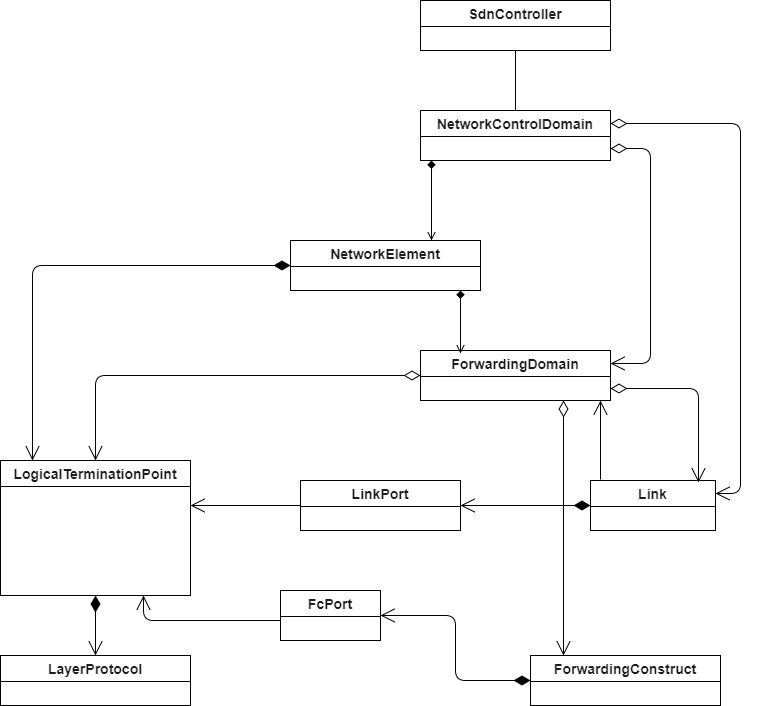
\includegraphics[width=1\textwidth]{core_model_uml_overview}
	\caption{Reprezentare UML simplificată a \textit{CoreModel}}
	\label{fig:core_model}
\end{figure}

O vedere de ansamblu simplificată, folosind \gls{uml} se poate vedea în Figura \ref{fig:core_model}. Blocurile relevante pentru simulatoarele dezvoltate vor fi detaliate în paragrafele următoare. Nu se vor detalia toate obiectele care alcătuiesc modelul informațional de bază deoarece, așa cum este sugerat în recomandarea \gls{onf}, modelul poate fi redus și simplificat, în funcție de nevoile pentru care este folosit.  

\subsection{Obiectul \textit{NetworkElement (NE)}}
%\paragraph{Network Element}

Obiectul \textit{NetworkElement} reprezintă un element de rețea - \gls{ne}, adică, în cazul \gls{sdn}, un echipament de dirijare din planul de date, sau, în cazul în care există virtualizare, un element virtual de rețea vizibil în interfaţa care folosește acea virtualizare.

Pentru o interfață directă între echipamentul de control \gls{sdn} către un echipament de rețea, obiectul \textit{NetworkElement} delimitează domeniul de control pentru resursele echipamentului, cum ar fi încapsularea folosită, multiplexarea, demultiplexarea, funcțiile asociate operaţiilor de administrare și de mentenanţă, etc. De asemenea, obiectul \textit{NetworkElement} defineşte domeniul spaţiilor de adresare pentru identificarea obiectelor care reprezintă resursele conţinute de echipamentul respectiv.

În cazul în care se folosesc metode de virtualizare, obiectul \textit{NetworkElement} reprezintă un element virtual de rețea. Asocierea unui element virtual cu unul real este responsabilitatea echipamentului de control \gls{sdn}. Cu ajutorul interfeţei de tip \textit{southbound} acesta poate crea sau şterge în mod dinamic astfel de obiecte pentru a oferi diferite vederi asupra rețelei, în funcție de nevoile aplicațiilor care se află deasupra echipamentului de control.

\subsection{Obiectele \textit{LogicalTerminationPoint (LTP)} și \textit{LayerProtocol (LP)}}

Obiectul \textit{LogicalTerminationPoint} - punct logic de terminaţie - cuprinde terminaţiile, adaptările sau funcțiile asociate operaţiilor de administrare și de mentenanţă ale unuia sau mai multor niveluri de transport. Prin natura sa, acest obiect suportă toate tipurile de protocoale, inclusiv cele pentru comutare de pachete sau pentru comutare de circuite. Fiecare nivel de transport este reprezentat de o instanţă a unui obiect \textit{LayerProtocol}, instanţă care poate fi folosită pentru a controla terminaţiile sau funcțiile de administrare și mentenanţă ale nivelului respectiv, sau pentru adaptarea (încapsularea sau multiplexarea semnalului client).

Dacă relația client-server între resursele echipamentului reprezentate de obiectele \textit{LTP} și \textit{LP} are un grad de asociativitate de 1:1 și este imuabilă, atunci un obiect \textit{LTP} poate conține mai multe obiecte \textit{LP}, de niveluri diferite de transport. Altfel, obiectele \textit{LP} de pe niveluri diferite trebuie să aibă asociate obiecte \textit{LTP} diferite.

Scopul acestor obiecte este acela de a oferi suport din perspectiva controlului și a administrării fără a fi nevoie de a defini atribute specifice unei anumite tehnologii, permițând astfel extinderea modelului fără a depinde de proprietățile tehnologiei respective, oferind flexibilitate sporită.

Un atribut important al obiectelor \textit{LP} este reprezentat de către \textit{layerProtocolName}. Acesta reprezintă nivelul de transport al obiectului și poate avea următoarele valori, conform \cite{onftr512v1.2}:

\begin{itemize}
	\item Nivel 0: \gls{ops}, \gls{ots}, \gls{oms}, \gls{och};
	\item Nivel 1: \gls{otu}, \gls{odu};
	\item Nivel 2: Carrier Ethernet: \gls{ety}, \gls{eth}; \gls{mpls-tp};
	\item Proprietăţi specifice nivelului de transport asociate cu obiectul \textit{LP}.
\end{itemize}

\subsection{Obiectul \textit{Forwarding Construct}}

Obiectele \textit{ForwardingConstruct (FC)} sunt folosite pentru a realiza dirijarea informației caracteristice nivelului de transport dat de obiectul \textit{LP} și oferă posibilitatea de a permite dirijarea între două sau mai multe obiecte \textit{LTP}. Astfel, obiectele \textit{FC} sunt independente de nivelul de transport folosit și suportă orice formă de pachete sau circuite.

Asocierea între \textit{FC} și \textit{LTP} se face prin port-uri, în care fiecare dintre acestea are un rol în contextul obiectului \textit{FC}. Dirijarea traficului între port-urile asociate se face în funcție de tipul de obiect \textit{FC}. Un astfel de obiect poate fi asociat unui singur obiect \textit{FD}. Ele pot fi definite recursiv (un obiect \textit{FC} poate fi parte din alt obiect \textit{FC}), însă la cel mai mic nivel de recursivitate acesta reprezintă de fapt o legătură în matricea de comutatoare a elementului de rețea.

Obiectele \textit{FC} pot fi folosite pentru a reprezenta orice fel de conexiune, cum ar fi punct la punct, punct la multi-punct sau multi-punct la multi-punct.

\subsection{Obiectul \textit{FC Port}}

Obiectele \textit{FC Port} sunt folosite, așa cum a fost prezentat anterior, la asocierea dintre obiectele \textit{FC} și \textit{LTP}. Dirijarea traficului între aceste obiecte se face conform tipului de \textit{FC}. De exemplu, \textit{FC Port} poate reprezenta un punct protejat (de încredere) sau un punct care protejează (de rezervă), în cazul în care rolul obiectului \textit{FC} este unul de protecție.

\subsection{Obiectul \textit{Forwarding Domain}}

\textit{ForwardingDomain} - domeniul de dirijare - este un obiect care modelează componenta topologiei care permite dirijarea pachetelor între diferite puncte ale resurselor echipamentului de rețea (reprezentate prin alte obiecte, de tipul \textit{LogicalTerminationPoint}). Lista punctelor logice de terminaţie care pot fi folosite de către un domeniu de dirijare este parte a acestui obiect. \textit{ForwardingDomain} poate conţine zero sau mai multe obiecte de tip \textit{ForwardingConstruct}, indiferent de nivelul la care se află acestea (Ethernet, MPLS, optic, etc.). 

Acest domeniu de dirijare oferă contextul pentru crearea, modificarea sau ștergerea obiectelor de tip \textit{ForwardingConstruct}. Obiectul \textit{ForwardingDomain} dintr-un element de rețea poate reprezenta comutatorul sau gruparea de comutatoare din echipamentul de dirijare.


\section{ONF TR-532 - Modelul informaţional pentru microunde (\textit{Microwave Information Model})}

Modelul informațional pentru microunde \cite{onftr532} a apărut in decembrie 2016 ca o recomandare formulată de grupul \gls{otwg} din cadrul \gls{onf}. Scopul acestuia este de a modela un echipament de transport de date fără fir, pentru a putea fi folosit de echipamentele de control \gls{sdn}, în încercarea de a asigura o independenţă față de producătorii de echipamente. Chiar dacă este denumit \textit{model informațional pentru microunde}, acesta poate fi aplicat fără probleme nu numai echipamentelor ce funcționează în spectrul microundelor, ci și echipamentelor care funcționează în benzi de frecvenţă mai înalte (lungimi de undă milimetrice), care încep să își facă tot mai mult simţită prezenţa în rețelele actuale de transport.

TR-532 este de fapt o extensie specifică tehnologiei \gls{wt} a modelului informațional de bază, versiunea 1.2 (TR-512.1). Legătura cu acesta se face prin extinderea clasei de obiecte \textit{\gls{lp}}. Astfel, modelul informațional pentru microunde conţine şase pachete condiţionale caracteristice tehnologiilor folosite pentru transport, care au în nume extensia \textit{*\_Pac}: 

\begin{itemize}
	\item \textit{MW\_AirInterface\_Pac};
	\item \textit{MW\_AirInterfaceDiversity\_Pac};
	\item \textit{MW\_PureEthernetStructure\_Pac};
	\item \textit{MW\_HybridMWStructure\_Pac};
	\item \textit{MW\_EthernetContainer\_Pac};
	\item \textit{MW\_TdmContainer\_Pac}
\end{itemize}

O imagine de ansamblu simplificată a acestui model, în limbajul \gls{uml}, care conţine doar obiectele relevante pentru simulatoarele dezvoltate, împreună cu legătura acestuia cu modelul informațional de bază este ilustrată în Figura \ref{fig:microwave_model}.

\begin{figure}[h]
	\centering
	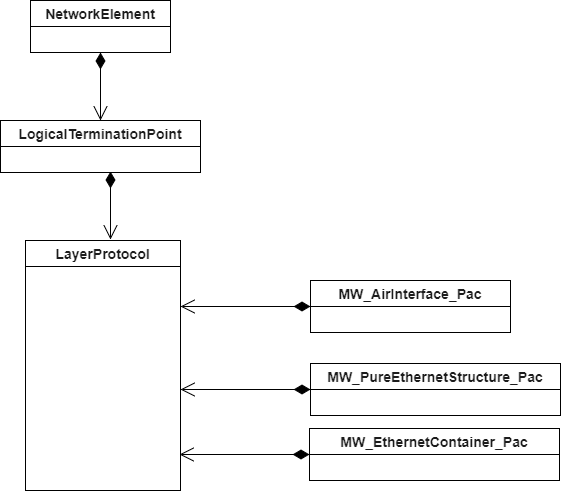
\includegraphics[width=1\textwidth]{microwave_model_overview}
	\caption{Reprezentare UML simplificată a \textit{MicrowaveModel} și legătura acestuia cu \textit{CoreModel} \cite{onftr532}.}
	\label{fig:microwave_model}
\end{figure}

În următoarele paragrafe se vor detalia obiectele acestui model care sunt importante din punctul de vedere al simulatoarelor dezvoltate în această lucrare.

\subsection{Obiectul \textit{MW\_AirInterface\_Pac}}

Obiectul \textit{MW\_AirInterface\_Pac} reprezintă o interfață radio fizică a unui echipament. Este denumit în recomandare ca \textit{punct de terminaţie a traseului secţiunii fizice de microunde} - \gls{mwps-ttp}, astfel că nivelul de transport al obiectului \textit{\gls{lp}} asociat este Secţiunea Fizică de Microunde - \textit{\gls{mwps}} \cite{onftr532}. O reprezentare simplificată în limbajul \gls{uml} a \textit{MW\_AirInterface\_Pac} se poate observa în Figura \ref{fig:airinterface_pac}.

\begin{figure}[h]
	\centering
	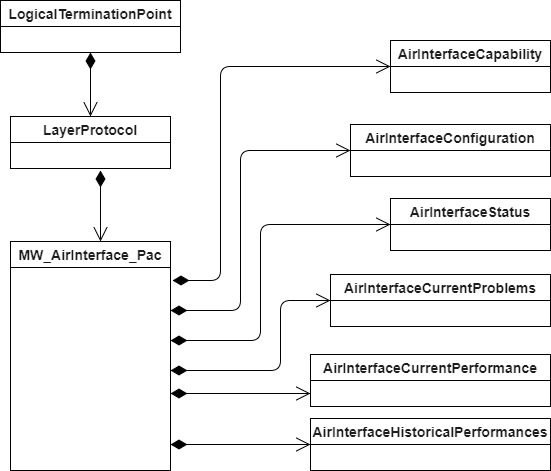
\includegraphics[width=1\textwidth]{airinterface_pac}
	\caption{Reprezentare UML simplificată a obiectului \textit{MW\_AirInterface\_Pac} \cite{onftr532}.}
	\label{fig:airinterface_pac}
\end{figure}

Acest obiect conţine alte câteva obiecte care modelează caracteristice unei interfețe radio fizice, cum ar fi: (i) capabilităţi ale modemului și ale transmiţătorului interfeţei radio asociate (de exemplu tipurile de modulaţie suportate pentru transmisie, valorile admisibile ale puterii de transmisie, intervalul de frecvenţe suportate de emiţător sau de receptor, alarmele expuse de interfață, suportul interfeţei pentru modulaţie adaptivă, etc.), (ii) parametrii configurabili ai interfeţei radio (de exemplu numele interfeţei, lărgimea de bandă a canalului de transmisie/de recepţie, frecvenţele folosite pentru transmisie/recepţie, puterea de transmisie, intervalul în care modulaţia poate lua valori, diferite alte caracteristici configurabile ale interfeţei, cum ar fi Anularea Interferenţei dintre Polarizări - \gls{xpic}, Intrări Multiple - Ieşiri multiple - \gls{mimo}, criptarea datelor, etc.), (iii) parametrii care descriu starea interfeţei la un anumit moment de timp (de exemplu frecvenţele actuale de transmisie/recepţie, nivelurile actuale de putere a semnalului de transmisie/recepţie, modulaţia actuală folosită, raportul semnal-zgomot măsurat de către modem, temperatura actuală a unităţii radio, etc.), (iv) problemele actuale ale interfeţei radio (adică alarmele care apar pe interfață la un moment dat), (v) valorile actuale ale parametrilor de performanţă a interfeţei și (vi) valorile istorice ale parametrilor de performanţă a interfeţei \cite{onftr532}.

\subsection{Obiectul \textit{MW\_PureEthernetStructure\_Pac}}

Obiectul \textit{MW\_PureEthernetStructure\_Pac} este o reprezentare logică a unei interfețe radio capabilă să transporte doar trafic Ethernet. Acest obiect este reprezentat într-un mod simplificat, în limbajul \gls{uml}, în Figura \ref{fig:pureethstructure_pac}. Asocierea cu o interfață fizică radio se face la nivelul modelului informațional de bază, printr-o relaţie de tip client-server.

\begin{figure}[h]
	\centering
	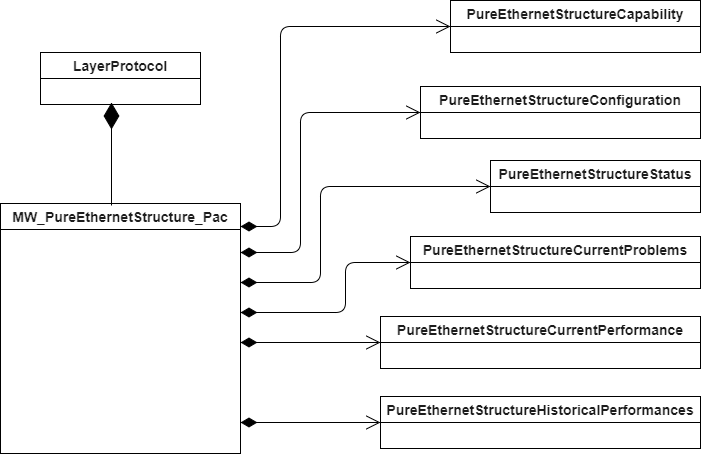
\includegraphics[width=1\textwidth]{pureethstructure_pac}
	\caption{Reprezentare UML simplificată a obiectului \textit{MW\_PureEthernetStructure\_Pac} \cite{onftr532}.}
	\label{fig:pureethstructure_pac}
\end{figure}

Acest obiect este denumit în recomandare ca \textit{punct de terminaţie a traseului secţiunii microunde} - \gls{mws-ttp}, astfel că nivelul de transport al obiectului \textit{\gls{lp}} asociat este Secținea de Microunde - \textit{\gls{mws}}. 

Structura obiectelor conţinute de către \textit{MW\_PureEthernetStructure\_Pac} este similară cu cea a obiectului \textit{MW\_AirInterface\_Pac}. Conţine obiecte care reprezintă (i) capabilitățile acestei interfețe logice (de exemplu alarmele aplicabile ei sau identificatorul structurii respective, care poate fi folosit de alte obiecte), (ii) parametrii configurabili ai interfeţei logice (de exemplu gradul de severitate a alarmelor pe care această interfață le expune), (iii) parametrii care descriu starea interfeţei logice la un anumit moment de timp, (iv) problemele actuale ale interfeţei logice, (v) valorile actuale ale parametrilor de performanţă a interfeţei logice și (vi) valorile istorice ale parametrilor de performanţă a interfeţei logice \cite{onftr532}.

\subsection{Obiectul \textit{MW\_EthernetContainer\_Pac}}

Obiectul \textit{MW\_EthernetContainer\_Pac} reprezintă de asemenea o interfață logică și este denumit în recomandare \textit{punct de terminaţie a conexiunii unui client de microunde}, pentru un semnal Ethernet client. Practic, este o interfață logică ce are rol de container pentru traficul Ethernet care este transmis de echipament prin radio. În raport cu obiectul \textit{\gls{lp}} acesta are un nivel de transport denumit Container Ethernet - \textit{\gls{etc}}. O reprezentare grafică simplificată în limbajul \gls{uml} a obiectului \textit{MW\_EthernetContainer\_Pac} poate fi găsită în Figura \ref{fig:ethcontainer_pac}.

\begin{figure}[h]
	\centering
	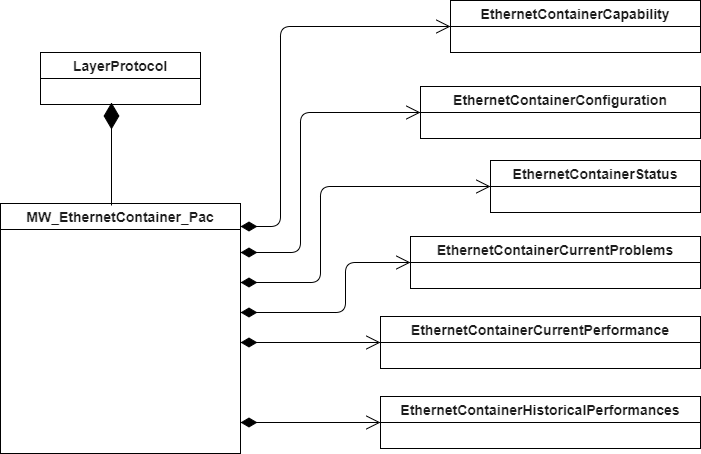
\includegraphics[width=1\textwidth]{ethcontainer_pac}
	\caption{Reprezentare UML simplificată a obiectului \textit{MW\_EthernetContainer\_Pac} \cite{onftr532}.}
	\label{fig:ethcontainer_pac}
\end{figure}

Și în cazul obiectului \textit{MW\_EthernetContainer\_Pac} se păstrează aceeaşi structura a obiectelor pe care le conţine, ca în cazul celorlalte două obiecte detaliate anterior. Astfel, acesta prezintă obiecte care reprezintă (i) capabilitățile containerului (de exemplu dacă există compresie la diferite niveluri, criptare a datelor sau alarmele pe care această interfață le expune), (ii) parametrii configurabili ai containerului (de exemplu un identificator al containerului, identificatoarele segmentelor folosite pentru a transporta traficul Ethernet asociat acestui container, etc.), (iii) parametrii care descriu starea containerului, (iv) alarmele la momentul actual de timp pe care containerul le raportează, (v) valorile actuale ale parametrilor de performanţă a containerului și (vi) valorile istorice ale parametrilor de performanţă a containerului \cite{onftr532}.
\section{Protocolul NETCONF}

Standardizare: ONF, etc..
\section{Alegerea unei soluții software pentru serverul NETCONF}

Există numeroase soluții care lucrează cu protocolul \gls{netconf}, atât pe partea de client, cât și pe cea de server. O listă a acestora este menţinută de către grupul de lucru \gls{netconf} și poate fi găsită online \cite{netconfwiki}. Conţine și soluții software proprietare, dar și soluții cu sursă deschisă. Pentru implementarea simulatoarelor prezentate în această lucrare au fost considerate trei opţiuni de implementare a unui server \gls{netconf}, cu sursă deschisă: \textit{Netopeer}, \textit{OpenYuma} și \textit{\gls{netconf} Test Tool} (unealtă oferită de proiectul \gls{odl}). O comparaţie între acestea va fi prezentată în continuare, justificând astfel alegerea de a folosi una dintre ele în simulatoare \cite{stancu2016comparison}.

\subsection{Netopeer}

\textit{Netopeer} este o soluție ce se bazează pe librăria \textit{libnetconf}, oferind atât o implementare pentru server, cât și una pentru un client al serverului. Această librărie este una cu sursă deschisă, implementată în limbajul C, ce oferă o implementare a protocolului \gls{netconf} \cite{krejci2013building}. Este o soluție care poate fi personalizată, oferind numeroase posibilităţi pentru implementările de server și de client și suportă toate caracteristicile protocolului \gls{netconf}.

\textit{Netopeer} oferă câteva unelte, de exemplu pentru a facilita integrarea modelelor informaționale \gls{yang} în module ale serverului, denumită \textit{administrator-netopeer - netopeer-manager}, sau pentru a configura caracteristicile serverului \gls{netconf}. Orice model de date \gls{yang} poate fi adăugat ca un modul al serverului, însă acesta trebuie prelucrat înainte. Astfel, fişierul \textit{*.yang} este transformat de către această soluție în fişiere pe care serverul le poate recunoaşte, inclusiv un fişier \textit{*.c}, care conţine un schelet de cod C, reprezentând așa-numite funcții cu apel invers (\textit{callback functions}) ce pot fi implementate pentru ca serverul să ofere comportamentul dorit, în raport cu modelul \gls{yang} folosit. Apoi, codul C este compilat, rezultând o bibliotecă partajată (\textit{shared library}) care poate fi utilizată de către codul de bază al serverului.

\subsection{OpenYuma}

\textit{OpenYuma} este o soluție software care se bazează pe proiectul \textit{Yuma}, care a devenit proprietar în anul 2011. Propune de asemenea implementări pentru server și client \gls{netconf}, scrise în limbajul C, oferind chiar posibilitatea de a încorpora acest cod în dispozitive al căror software folosește tot limbajul C.

\textit{OpenYuma} are o filosofie asemănătoare cu \textit{Netopeer}, oferind unelte pentru transformarea modelelor \gls{yang} în cod C schelet, care să fie apoi implementat pentru ca serverul \gls{netconf} să ofere facilităţile propuse. Unealta propusă de această soluție software se numeşte \textit{yangudmp} și transformă fişierele \textit{*.yang} în fişiere \textit{*.h} și \textit{*.c}, conţinând, la fel ca în cazul \textit{Netopeer}, funcții de apel invers ce trebuie rescrise.

Codul C obţinut după transformarea modelelor \gls{yang} se compilează, rezultând tot o bibliotecă partajată care să poată fi folosită de către codul de cază al serverului. Aceasta poate fi încărcată în momentul inițializării serverului sau chiar în mod dinamic, în timp ce acesta rulează.

\subsection{Unealta de Test Netconf - \textit{Netconf Testtool}}

Unealta de Test Netconf este o soluție software oferită în cadrul proiectului OpenDaylight \cite{odlnetconftesttool}. Este o soluție simplă, care nu poate fi personalizată foarte mult, oferind doar o implementare Java pentru un server \gls{netconf}. Aceasta este folosită de proiectul \gls{odl} pentru a-și testa interfaţa de Sud care implementează protocolul \gls{netconf}.

Scopul acestei soluții este puţin diferit de al celorlalte, deoarece \textit{Testtool} nu își propune oferirea unei soluții software care implementează un server \gls{netconf} care apoi să poată fi integrat cu echipamentele de rețea, ci oferirea unei soluții simple și rapide care să încarce un model \gls{yang} specific, cu scopul de a-l testa. Cu toate acestea, acest software a fost considerat pentru comparaţie, deoarece și scopul simulatoarelor este de a testa modelele \gls{yang} și de a crea topologii specifice rețelelor de transport de date fără fir, expunând modelele informaționale descrise anterior.

\subsection{Comparaţie între soluţiile care oferă server NETCONF}

Soluţiile descrise anterior au fost evaluate atât prin compararea documentaţiei relevante pe care acestea o pun la dispoziţie, cât și prin experimente practice care iar în considerare diferite scenarii. 

Comparaţia bazată pe lucrurile descrise în documentaţie este rezumată în Tabelul \ref{tab:Table_1}, în timp ce un sumar al comparaţiei bazată pe experimentare se găseşte în Tabelul \ref{tab:Table_2}.

\begin{table}[hp]
	\caption{Comparaţie a caracteristicilor oferite de cadrele software considerate.\label{tab:Table_1}}
	
	\begin{tabular}{|M{0.35\textwidth}|M{0.17\textwidth}|M{0.17\textwidth}|M{0.16\textwidth}|}
		\hline 
		\textbf{Criteriile} & \multicolumn{3}{c|}{\textbf{Soluții servere NETCONF}} \tabularnewline
		\cline{2-4} 
		\textbf{de comparație} & \textbf{\emph{Netopeer}} & \textbf{\emph{OpenYuma}} & \textbf{\emph{Testtool}}\tabularnewline
		\hline 
		Limbajul de programare & C & C & Java\tabularnewline
		\hline 
		Încărcarea modelelor YANG brute & Nu & Nu & Da\tabularnewline
		\hline 
		Încărcarea dinamică a modulelor în server & Da & Da & Nu\tabularnewline
		\hline 
		Baza de stocare a datelor NETCONF & toate & toate & de operare \tabularnewline
		\hline 
		Suport pentru notificări & da & da & da\tabularnewline
		\hline 
		Port configurabil & da & da & da\tabularnewline
		\hline 
		Mai multe instanțe de server & nu & da & da \tabularnewline
		\hline 
		Mai multe conexiuni în același timp & da & da & da\tabularnewline
		\hline 
		Capabilități pentru depanare & jurnalizare & jurnalizare & jurnalizare\tabularnewline
		\hline
	\end{tabular}
\end{table}

Primul criteriu care poate fi considerat este limbajul pe programare în care aceste soluții software sunt implementate: \textit{Netopeer} și \textit{OpenYuma} sunt scrise în limbajul C, pe când \textit{Testtool} este o implementare Java.

Un alt criteriu pentru evaluare constă în abilitatea serverului de a încărca în mod direct (dinamic sau în momentul inițializării) modele \gls{yang}. Această posibilitate este oferită doar de implementarea Java. Celelalte două soluții au nevoie de o fază premergătoare de procesare,transformând fişierele \textit{*.yang} în \textit{*.c}. \textit{Netconf Test Tool} poate încărca modelul \gls{yang} doar în momentul inițializării serverului, dintr-un director anume, pe când celelalte cadre software pot încărca acest model, după ce a fost procesat, în mod dinamic.

Un alt subiect pentru comparaţie este dat de tipurile de baze de stocare de date propuse de protocolul \gls{netconf} suportate de implementările serverelor. \textit{Netopeer} și \textit{OpenYuma} folosesc fişiere \gls{xml} în care stochează informaţiile și suportă toate cele trei tipuri de baze de stocare a datelor propuse de \gls{netconf}: de iniţializare, de rezervă și de operare. Cealaltă soluție software, \textit{Testtool} oferă posibilitatea de a utiliza doar baza de stocare de date de operare stocând valorile parametrilor în variabile de execuţie, acestea pierzându-se în momentul în care serverul este oprit. O diferenţă importantă apare în acest context, între cele două soluții implementate în C, \textit{OpenYuma} oferind o flexibilitate mai mare. În cazul \textit{Netopeer}, atunci când serverul se iniţializează, încarcă valorile parametrilor din bazele de stocare de date de iniţializare și de operare în memorie. Apoi, începe să analizeze valorile din baza de stocare de date de iniţializare, comparându-le cu valorile corespunzătoare atributelor din cea de operare. Dacă valorile nu sunt egale, sau valoarea din baza de stocare de date de operare nu există (însemnând prima utilizare a serverului), atunci serverul copiază valoarea din baza de stocare de date de iniţializare și apelează funcţia de apel invers asociată parametrului de configurare. Prin această abordare severul se asigură ca nu există inconsistenţe între bazele de stocare de date de iniţializare și de operare și, mai mult, dacă acest server este conectat la un echipament real de rețea, prin apelarea funcţiei cu apel invers asociate parametrului, dispozitivul va fi configurat astfel încât valorile din server să reflecte valorile de pe echipament. \textit{OpenYuma} are o abordare mai flexibilă, permiţând dezvoltatorilor să altereze baza de stocare de date de operare în timpul inițializării modulului, fără a implica baza de stocare de date de iniţializare.

\begin{table}[tp]
	
	\caption{Compararea practică a cadrelor software considerate\label{tab:Table_2}}
	\begin{tabular}{|M{0.35\textwidth}|M{0.17\textwidth}|M{0.17\textwidth}|M{0.16\textwidth}|}
		\hline
		\textbf{Scenariul experimentat} & \textbf{\emph{Netopeer}} & \textbf{\emph{OpenYuma}} & \textbf{\emph{Testtool}} \tabularnewline
		\hline 
		Procesarea \textit{*.yang} în \textit{*.c} & lnctool & yangdump & N/A\tabularnewline
		\hline 
		Reprezentarea bazei de stocare a datelor în cadrul serverului & fişier XML & fișier XML & variabile de execuție \tabularnewline
		\hline 
		Încărcarea datelor în faza de iniţializare a serverului & \textit{startup} & flexibilă, orice se poate suprascrie & N/A \tabularnewline
		\hline 
		Implementarea notificărilor NETCONF & \textit{libnetconf} & funcție cu apel invers oferită & fișier XML \tabularnewline
		\hline 
		Funcții pentru parametrii configurabili & câte una per atribut & câte una per atribut & N/A\tabularnewline
		\hline 
		Funcții pentru parametrii de stare & doar una, globală & câte una per atribut & N/A\tabularnewline
		\hline 
		Conexiuni concurente de la clienți & da & suportă, trebuie implementat & da\tabularnewline
		\hline \end{tabular}
\end{table}

O altă caracteristică importantă a serverelor care poate fi comparată este abilitatea de a genera notificări \gls{netconf}. Toate cele trei soluții oferă notificări. În cazul \textit{Testtool} este o implementare simplă, acestea fiind declanşate printr-o comandă \gls{netconf} și trimise dintr-un fişier \gls{xml} care le conţine. \textit{OpenYuma} oferă câte o funcție cu apel invers pentru fiecare notificare pe care o găseşte în momentul procesării modelului \gls{yang}. \textit{Netopeer} nu are această abilitate în mod implicit, însă suportul este oferit de \textit{libnetconf}.

Din perspectiva funcţiilor cu apel invers generate în momentul procesării modelului \gls{yang} putem compara doar cele două soluții implementate în limbajul C, deoarece \textit{Testtool} nu oferă astfel de caracteristici. Soluția \textit{Netopeer} oferă posibilitatea de a alege care dintre parametrii configurabili vor avea o funcție cu apel invers asociată, în timp ce \textit{OpenYuma} va genera o astfel de funcție pentru fiecare din parametrii configurabili pe care îi găseşte în modelul \gls{yang}. Pentru informaţiile de stare \textit{Netopeer} generează o singură funcție cu apel invers care este apelată pentru orice operaţie \gls{netconf} de tip \textit{get} care ajunge la server, iar \textit{OpenYuma} generează câte o astfel de funcție pentru fiecare parametru de stare.

Din punctul de vedere al abilităţii de a configura portul pe care serverul acceptă conexiuni, toate soluţiile oferă această posibilitate. \textit{Testtool} are nevoie de un port de plecare, incrementând apoi numărul portului pentru celelalte instanţe ale serverului. Și celelalte soluții oferă posibilitatea de a schimba portul pe care serverul ascultă. Din perspectiva rulării mai multor instanţe de server pe aceeaşi mașină, atât \textit{Testtool} cât și \textit{OpenYuma} oferă această posibilitate, diferitele instanţe folosind porturi diferite. \textit{Netopeer}, pe de altă parte, nu permite rularea mai multor instanţe pe aceeaşi mașină.

Un alt criteriu pentru compararea acestor cadre software este dat de suportul pentru mai multe fire de execuție, adică abilitatea serverului de a permite conectarea mai multor clienţi în același timp. \textit{Testtool} oferă această posibilitate. \textit{OpenYuma} oferă de asemenea acest suport, cu menţiunea că accesul concurent la resursele comune trebuie rezolvat în funcțiile cu apel invers care vor fi implementate de către dezvoltatori, nefiind rezolvat de către cadrul software. În cazul \textit{Netopeer}, acest acces concurent este rezolvat din faza de proiectare a serverului și este oferit de \textit{libnetconf}.

Și capabilitățile de depanare oferite ar putea constitui un criteriu de comparaţie, însă toate soluţiile se bazează pe fişiere de tip jurnal, oferind mai multe niveluri de jurnalizare.

Pe baza acestei comparaţii a fost aleasă soluţia \textit{OpenYuma} pentru implementarea serverului \gls{netconf} folosit în simulatoare, ea oferind cea mai mare flexibilitate.
\section{Arhitectura demonstraţiilor de concept WT SDN}

Standardizare: ONF, etc..
